\documentclass[acmtog]{acmart}
\usepackage{graphicx}
\usepackage{subfigure}
\usepackage{natbib}
\usepackage{listings}
\usepackage{bm}
\usepackage{amsmath}

\definecolor{blve}{rgb}{0.3372549 , 0.61176471, 0.83921569}
\definecolor{gr33n}{rgb}{0.29019608, 0.7372549, 0.64705882}
\makeatletter
\lst@InstallKeywords k{class}{classstyle}\slshape{classstyle}{}ld
\makeatother
\lstset{language=C++,
	basicstyle=\ttfamily,
	keywordstyle=\radiance{blve}\ttfamily,
	stringstyle=\radiance{red}\ttfamily,
	commentstyle=\radiance{magenta}\ttfamily,
	morecomment=[l][\radiance{magenta}]{\#},
	classstyle = \bfseries\radiance{gr33n},
	tabsize=2
}
\lstset{basicstyle=\ttfamily}

% Title portion
\title{Final project: {Multi-Resolution Isosurface Rendering}}

\author{Name:\quad QiYukun  \\ student number:\ 2020533002
	\\email:\quad qiyk@shanghaitech.edu.cn\\}
\author{Name:\quad DiHaichuan  \\ student number:\ 2020533116
	\\email:\quad dihch@shanghaitech.edu.cn}

% Document starts
\begin{document}
	\maketitle
	
	\vspace*{2 ex}
	
	\section{Introduction}
	\begin{itemize}
		\item Brief introduction of related paper.
		\item Basic task of this project.
		\item Load VDB data.
		\item Direct volume rendering.
		\item Data travsersal in multi-resolution grids.
		\item Interpolation.
		\item Classification.
		\item Some other tasks.
	\end{itemize}
	\section{Implementation Details}
	\subsection{Brief introduction of related paper.}
	In [2021] Ray Tracing Structured AMR Data Using ExaBricks, this paper designs a techonolgy of data to enable simulations to adapt the domain resolution to save computation and storage, which is called Adaptive Mesh Refinement(AMR). This techonolgy adapts the sampling rate to the corresponding cell size and when overlap happens it will choose the finer resolution. It can also skip some empty area.
	\subsection{Basic task of this project.}
	The task of this project is to rendering four given data efficiently and beautifully. The four given data are VDB files which store results of fluid simulations. Two of them are single-resolution and two others are multi-resolution and have overlap of different resolution. Because the VDB files store a velocity field which is a vector field , we need to convert it to a scalar field to visualize it. For example, we can convert the vector field into a speed field or use Q-criterion.
	\subsection{Load VDB data.}
	In a VDB file, it contains one or more uniform girds and each uniform grid may have different resolution. Between uniform grids, there may have overlaps. In one unform gird, every cells have the same size and some cells may be empty. In metadata of a VDB file, every cells' location is contained by an origin cell's bottom front left corner world location and cell's local coordinate and gird size.In this project, we use library OpenVdb to load in VDB files.
	\subsection{Direct volume rendering.}
	There are many ways to visualize volume data. In this we choose the most directly way. We use direct volume rendering method. In this method, we generate rays to traverse the girds, and then calculate the approximate value by interpolation. If the value is in the data range we need, we give it a color based on its value, and use volume rendering to show layers of data. In our method, we think that there are vacuum between two satisfied data, so transparency will be only determined by how many layers of data it has hit not by distance.    
	\subsection{Data traversal in multi-resolution grids.}
	In library OpenVdb, it gives a function to do data traversal, however the function only make sure that it will march a grid but not make ensure the step length is same. Thus, we write a our own function to do data traversal. In this function, the step is decided by the resulotion of the grid and it will skip choose the finer one when overlap happens. Also, our function can skip empty grids.
	\subsection{Interpolation.}
	In each cell, it contains the value of its bottom front left corner, so we need to do interpolation.
	Basicly, we can use three-linear interpolation, which do linear interpolation on line, surface and volume of nearby 2X2X2 data. However, it will cause stripe of girds on the result. Thus, we use
	cubic B-spline interpolation, which use nearby 4X4X4 data.
	\subsection{Classification.}
	We decide the color by the value of interpolation by the function Color = $ (value^{-0.3},1-value^{-0.3},0) $ and convert it into a integer vector in range of [0,255].
	\subsection{Some other tasks.}
	We use super-scaling method to do anti-aliasing and use BVH tree to store the mesh of sphere.
	\section{Results}
	% pictures should be in
	\begin{figure}[ht]\centering 
		\subfigure[Figure1]{
			\centering
			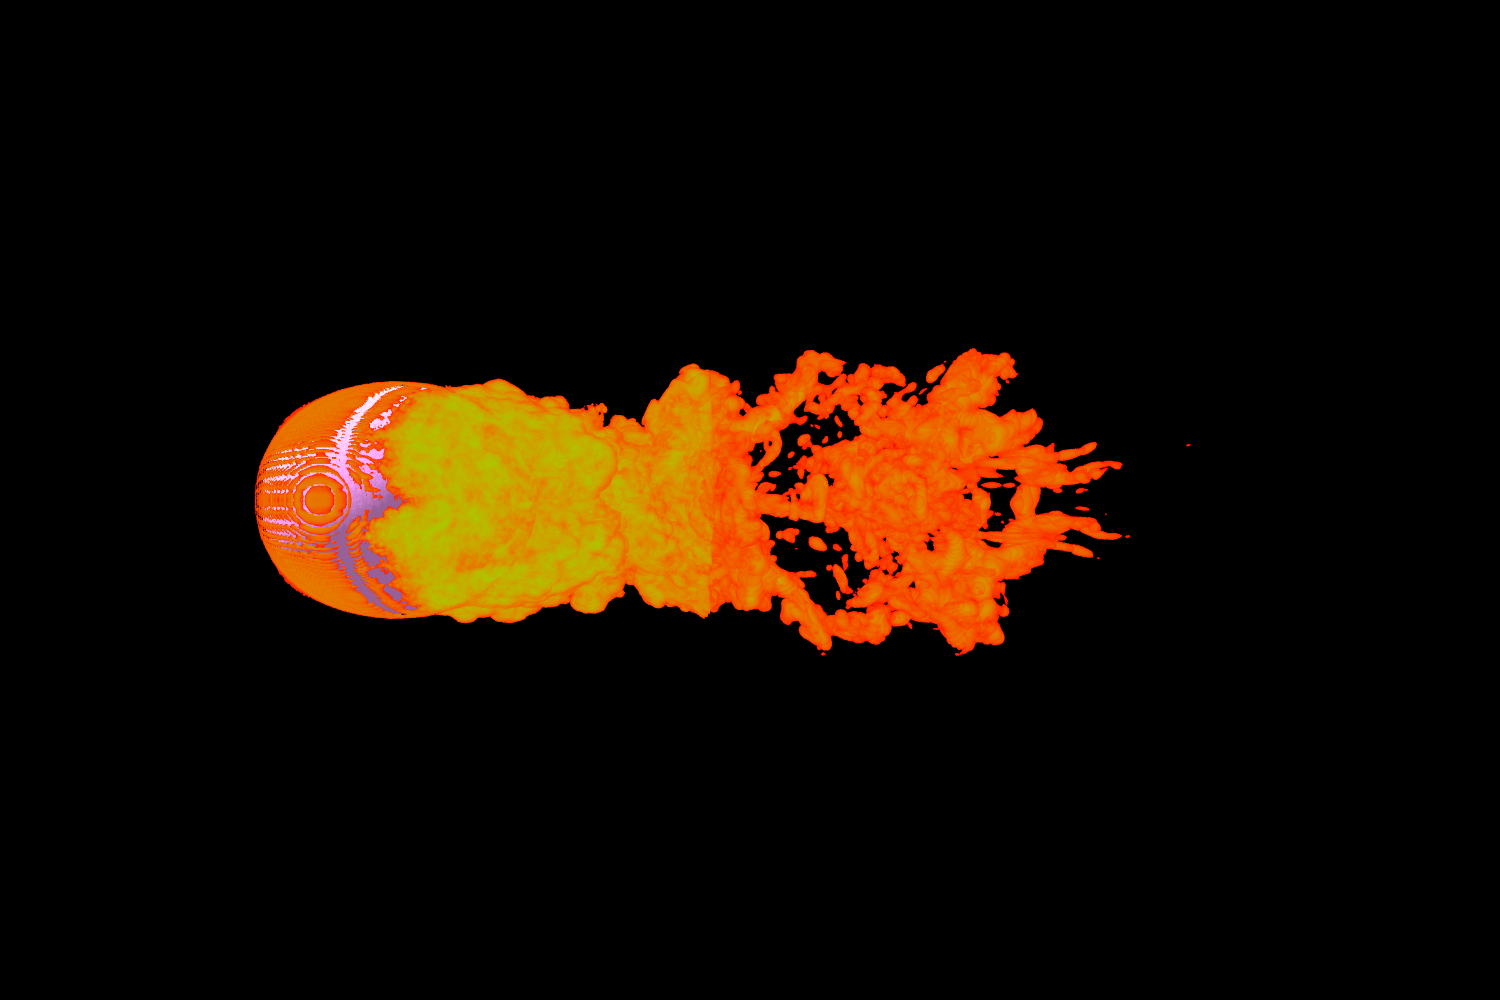
\includegraphics[height=3.5cm,width=5.25cm]{result-bspline-trans10.png}
		}\\
		\label{Figure1}
	\end{figure}
	\begin{figure}[ht]\centering 
		\subfigure[Figure2]{
			\centering
			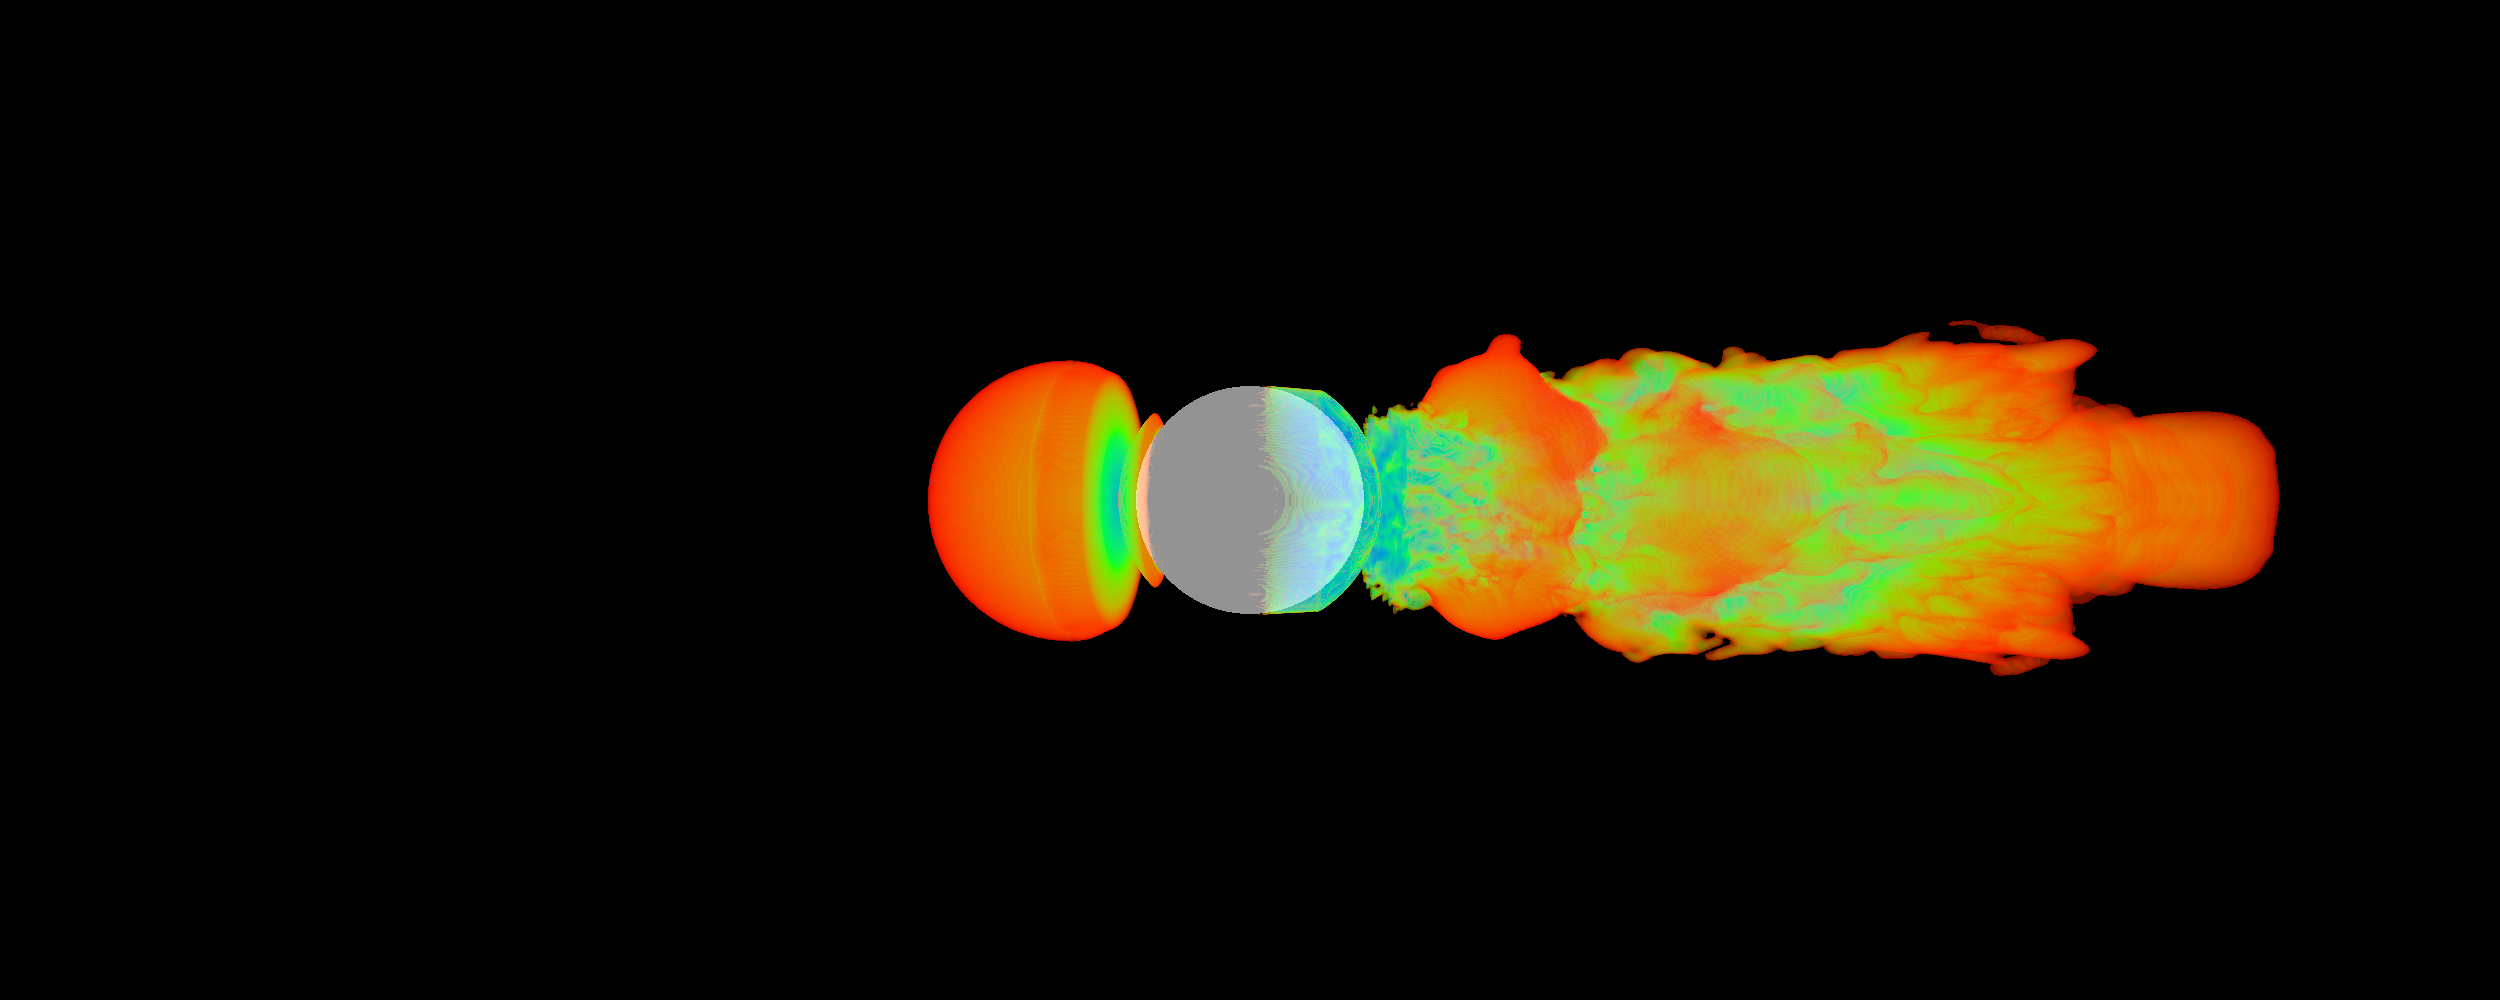
\includegraphics[height=3.5cm,width=8.75cm]{result-velomodel.png}
		}\\
		\label{Figure1}
	\end{figure}

	
\end{document}
